In order to immerse the player in the game, previously described core gameplay mechanics are further enhanced by visual, auditory and tactile feedback. This is done by using additional hitsounds, visual effects, or in the case of arcade cabinets, through decorations around the cab. As a result, it is easier for the player to get into the flow state -- a state of mind where the player is fully immersed in the game and is able to perform at their best. Additionally, in that state the player obtains the most enjoyment from the performed activity. As Jenova Chen says in his MFA thesis \cite{chen2006flow}:
\begin{quote}
    People associate many feelings with "fun": the sense of timelessness, of being at one, of exhilaration, focus, immediacy. (...)
    
    There is universal agreement that without a dynamic balance between the challenge of an activity and the ability to meet that challenge, fun is something we are definitely not having. Interestingly, making it possible for anyone to find exactly the right amount of challenge to engage with the exact abilities is the only way to access Flow. This means that when work is fun we have created complex, but negotiable challenges, challenges that allow the individual to engage or disengage, to work harder or work safer. [Dekoven DeepFun.com]
    
    At this point, fun can be defined as Flow, a balance of the relationship between challenge and ability (Chen 2006: 7).
\end{quote} 
As the player can adjust the desired difficulty level, it is easy to find the perfect balance between the challenge and player's ability to meet it. This is the reason why rhythm games are accessible for both beginners and advanced players, who are familiar with the genre already. In both cases, the gameplay and game design provide good conditions for the player to get into the flow state. No matter the skill of the player, elements of the gameplay, UI and auditory feedback play a crucial part in the immersion and entering the flow state. Described feedback is especially visible in \textit{Beat Saber} -- a Virtual Reality rhythm game, where the player is fully transferred into the game world through VR headset and controllers. The gameplay of \textit{Beat Saber} tracks the movement of the player's body and controllers which are held in both hands, requiring the player to slice approaching notes with two swords (controllers) and avoid obstacles by actually moving their body. Upon slicing the notes, the game provides auditory, haptic (using the vibration of controllers) and visual feedback -- the sight and sound of the note being cut in half inform that the note had been correctly cut, providing the instant response matching the rhythm of the currently played song. While being surrounded by the game world in VR, the score and combo counter is shown to the player during the gameplay, making it possible to keep track of the performance during gameplay. As every other rhythm game, the player can start by playing easy levels and understand the basic mechanics of the game, grasping its rules through the observation of the outcome and instant feedback. The game's UI is intuitive -- for example, the notes which are approaching the player have an arrow which indicates the required direction of the slice. If this mechanic is too difficult for beginners, it is possible to turn on the no-fail mode or make the notes possible to slice from all directions. This way, the game is accessible for the most novice players who also need to get used to VR and controllers.

\begin{figure}[h]
    \centering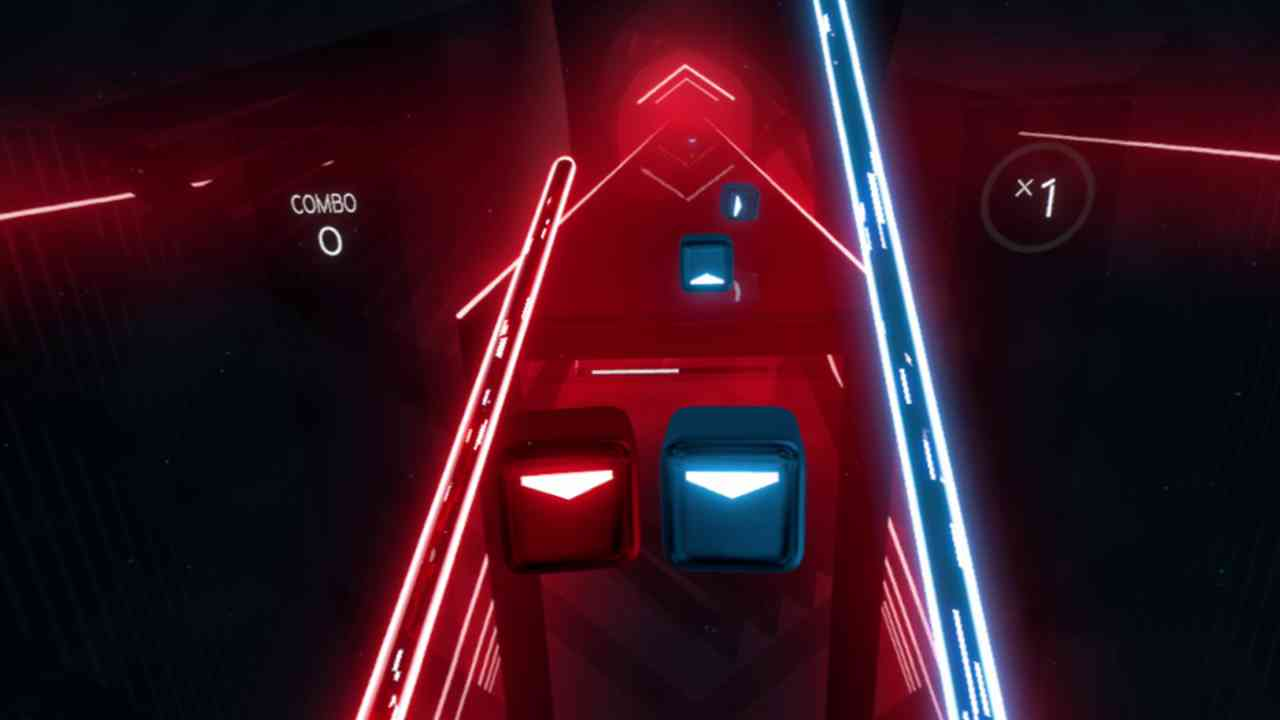
\includegraphics[scale=0.2]{obrazki/beatsaber.jpg}
    \caption{\textit{Beat Saber} -- screenshot of the gameplay. The red notes are corresponding to the sword held in the left hand, and the blue ones which correspond to the sword held in the right hand. The arrows placed on the notes are indicating the direction of slicing. \cite{beatsaber}}
    \label{fig:beatsaber}
\end{figure}

Fares Kayali emphasises this aspect of immersion in his thesis \cite{faresplayingmusic}:

\begin{quote}
    When designing a game, one must focus on the experience of the player and his or her involvement with the game. Ideally, an immersive game experience suspends the player in a state of flow. Being immersed and acting in flow with a game world leads the player to a "willing suspension of disbelief", a mental state first described by Samuel Taylor Coleridge (1817) in relation to literature and the reader. It signifies the willingness of the reader (or in this case the player) to "buy into" the prepared fictional world, putting aside rational doubts about its authenticity. The recipient suspends disbelief, diving into the presented world and greatly raising involvement. To enhance this state of immersion, a fictional world must provide a consistent setting that does not disrupt this willing suspension of disbelief (Kayali 2008: 112).
\end{quote}

Through immersing the player fully into the game world by the Virtual Reality, the experience of \textit{Beat Saber} is more likely to put these rational doubts of the player aside, enhancing the player's focus and commitment to the gameplay. Moreover, the \textit{Beat Saber}'s feedback is satisfying and rewarding, making the world presented in Virtual Reality more consistent with the musical experience.
Another example of such usage of feedback is \textit{SOUND VOLTEX} -- an arcade rhythm game developed and published by BEMANI, featuring a unique controller with four main buttons placed in the middle, two wide buttons placed below main buttons and two knobs placed on the sides of the controller.

\begin{figure}[h]
    \centering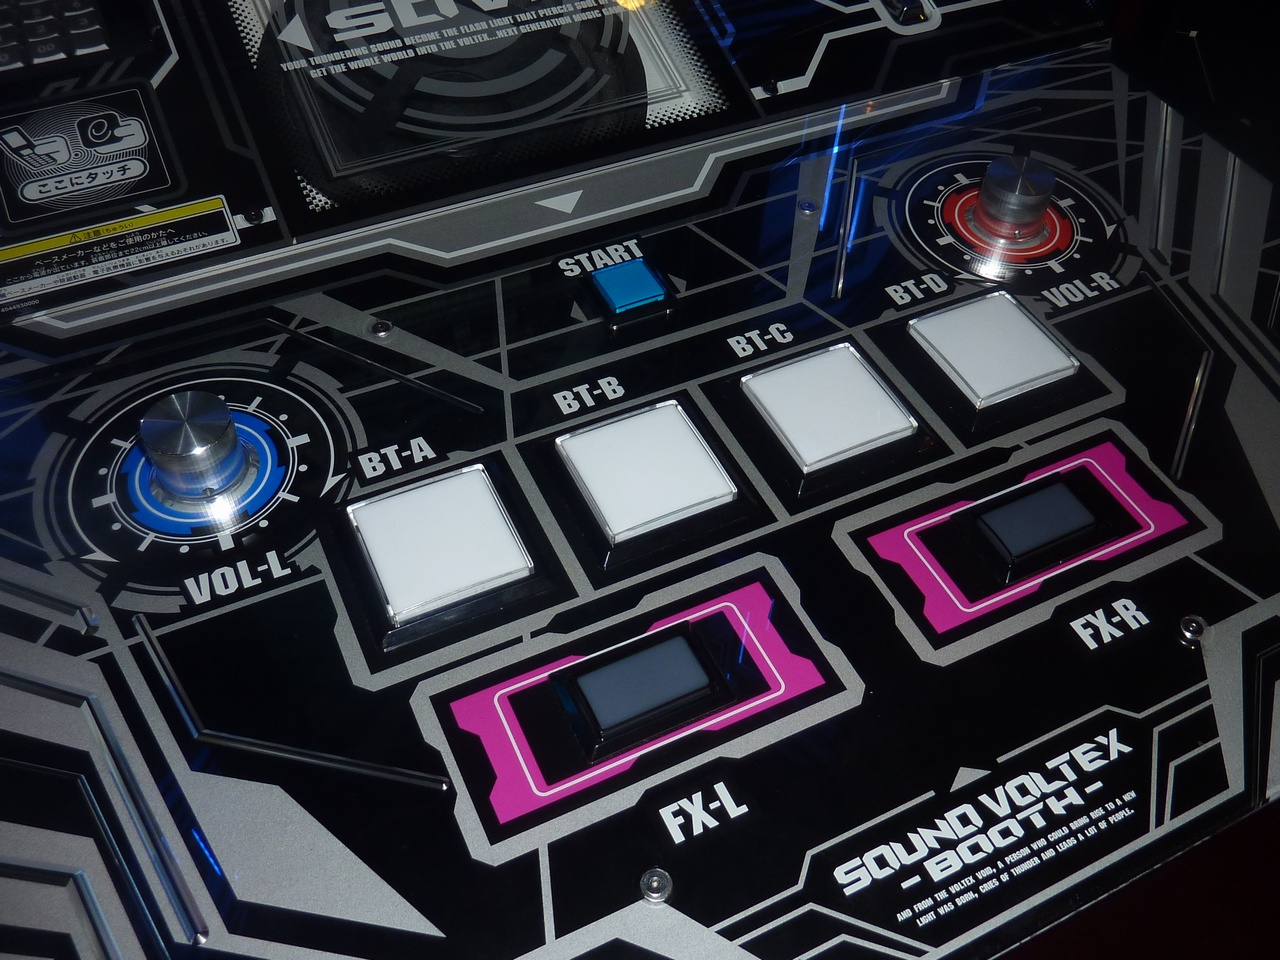
\includegraphics[scale=0.5]{obrazki/sdvxcontroller.jpeg}
    \caption{\textit{SOUND VOLTEX} Controller -- the composition of its controller makes it stand out from other rhythm games cabinets.\cite{sdvxcontroller}}
    \label{fig:sdvx}
\end{figure}

Once the player has chosen a track from the list and the difficulty of the chart (song), the game is played on a vertically scrolling road with 6 segments with aforementioned notes that correspond to the physical buttons. The gameplay consists of 3 types of notes: Basic white notes that appear in the middle 4 segments, corresponding to the white buttons; Orange notes which appear beneath white notes and cover 2 middle segments - corresponding to the wide buttons placed on the bottom of the controller; Two lasers marked with vivid colors: Blue (left knob) and pink (right knob) that appear on the outer segments of the road. In order to better understand the game and distinguish types of notes, the buttons on the controller are signed with names: knobs are named VOL-L (left) and VOL-R (right), names BT-A, BT-B, BT-C, BT-D for white main ones, and FX-L and FX-R names for bottom, wide buttons. Thanks to the arrangement of the controller's buttons and vivid colors of notes showed during the gameplay, the player can easily get used to reading the chart and hitting the corresponding buttons. As the note reaches the judgement line (above the representation of the controller), the player can see the accuracy of the hit -- the note is judged as CRITICAL, NEAR or MISS. The game also features a lifebar, which goes up as the notes are hit to the rhythm, or decreases if missed. In order to pass the chart the player must exceed the particular level of health bar (which differ from one difficulty to another). If the player is missing too many notes, it causes the song to CRASH, ending the course. Moreover, the buttons of \textit{SOUND VOLTEX} controller are satisfying to use, as they light up and give a firm, tactile response with a satisfying "click" upon pressing. On top of that, the modern design of the game's cabinet and controller matches the futuristic aesthetic of the game, presented in the game's gameplay, UI, illustrations and featured music, which includes many genres but revolves mostly around electronic genres. The game's menu features characters in anime-style illustrations, with sci-fi inspired outfits, accessories and hairstyles, matching the futuristic aspects of the game. 

\begin{figure}[h]
    \centering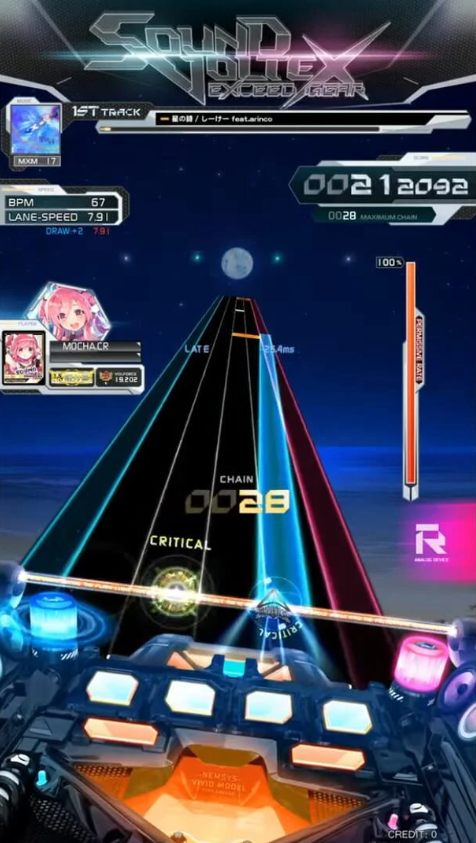
\includegraphics[scale=0.4]{obrazki/sdvx.png}
    \caption{\textit{SOUND VOLTEX} -- screenshot of the gameplay. The player is required to press the buttons and turn the knobs in the rhythm of the song. In this screenshot, the one can see the blue laser note which requires the player to turn the knob from left to right, which is further followed up by pressing up the orange note and then the white one. \cite{sdvx}}
    \label{fig:sdvx2}
\end{figure}

The auditory feedback of \textit{SOUND VOLTEX} is especially important regarding the immersion of the game. Similarly to \textit{beatmania}, \textit{SOUND VOLTEX} introduces audio effects upon every input made by the player through the controller. Every hit of the note and following the laser notes are mixing the original version of the song played, providing new experience from listening to it. As one song usually have few difficulties to play, the same song can have several remixes based on the density of notes to hit. The laser notes are making this experience even more immersive, as the "laser" sound produced by turning the knob is different depending on the direction of the turn and the speed rate. It comes along with the visual feedback of the game, as the whole stage is rotating accordingly to the knobs input. Such aspect is heightened when clearing sharp turns, in which the laser line crosses the road horizontally -- such laser notes require the player to turn the knob quickly, producing intense swishing sound effect that comes along with whole 360 degree spin of the scene. On the other hand, long orange notes that requires the player to hold the wide buttons are used to produce a sound effect that resembles a DJ turntable scratch. During the gameplay, the stage also zooms in or out to enhance the particular moments of the song -- such as more melodic or build-up parts with many notes to hit. It enhances the player's experience and makes the chart easier to read, as zooming out shows more of the upcoming notes. Adding the haptic feedback which is produced by the controller's buttons, the player can feel as they are actually performing and remixing the currently playing song.
Such connection of the visual, auditory and haptic feedback, plays a crucial part in immersing the player and evoking the flow state. As the feedback makes the gameplay more satisfying and enhances the rhythm, it is more likely for the player to enter the flow state, while enjoying the game to the fullest. Such experience provides better environment to focus on the play, as the fully immersion makes the game easier to learn and master the player's skills. 

As Mihaly Csikszentmihalyi says in his book \textit{Flow: The Psychology of Optimal Experience} \cite{csikszentmihalyi1990flow}:
\begin{quote}
    As our studies have suggested, the phenomenology of enjoyment has eight major components. (...) First, the experience usually occurs when we confront tasks we have a chance of completing. Second, we must be able to concentrate on what we are doing. Third and fourth, the concentration is usually possible because the task undertaken has clear goals and provides immediate feedback. Fifth, one acts with a deep but effortless involvement that removes from awareness the worries and frustrations of everyday life. Sixth, enjoyable experiences allow people to exercise a sense of control over their actions. Seventh, concern for the self disappears, yet paradoxically the sense of self emerges stronger after the flow experience is over. Finally, the sense of the duration of time is altered; hours pass by in minutes, and minutes can stretch out to seem like hours. The
    combination of all these elements causes a sense of deep enjoyment that is so rewarding people feel that expending a great deal of energy is worthwhile simply to be able to feel it (Csikszentmihalyi 1990: 57).
\end{quote}

Analysing aforementioned \textit{SOUND VOLTEX} mechanics and feedback regarding this quote, it is easy to observe how the game evokes the flow state. The provided satisfaction from the play is ensured by engaging the player in the task that may be completed in deep focus state -- starting from the ability to choose favorite song and the desired difficulty, followed by the instant feedback and responsible mechanics during the gameplay, ending the course with results, score and the feeling of accomplishment. Such design of the player's experience provides a great environment that enhances the player's engagement, supporting the ability to learn and master the game. Taking all of the described elements into the account, it is clear that elements that enhance the immersion are concomitantly evoking the flow state.